\begin{figure}[tbp]
  \centering
  \begingroup
  \definecolor{coreblue}{RGB}{48,91,120}
  \definecolor{coreorange}{RGB}{163,92,43}
  \resizebox{0.95\linewidth}{!}{%
  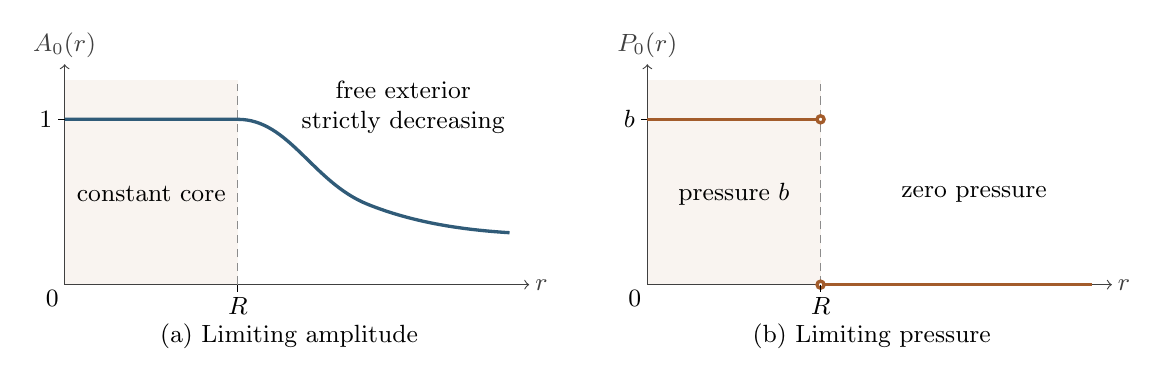
\begin{tikzpicture}[
    x=1cm,y=1cm,font=\small,
    axis/.style={->,thin,black!75},
    guide/.style={densely dashed,thin,black!45},
    amplitude/.style={very thick,coreblue},
    pressure/.style={very thick,coreorange},
    every node/.style={inner sep=2pt}]
    \begin{scope}
      \fill[coreorange!7] (0,0) rectangle (2.2,2.6);
      \draw[axis] (0,0) -- (5.9,0) node[right] {$r$};
      \draw[axis] (0,0) -- (0,2.8) node[above] {$A_0(r)$};
      \draw[guide] (2.2,0) -- (2.2,2.55);
      \draw[amplitude] (0,2.1) -- (2.2,2.1)
        .. controls (2.85,2.1) and (3.15,1.3) .. (3.85,1.02)
        .. controls (4.4,.8) and (5.0,.7) .. (5.65,.66);
      \draw (0,2.1) -- (-.08,2.1) node[left] {$1$};
      \draw (2.2,0) -- (2.2,-.09) node[below] {$R$};
      \node[below left] at (0,0) {$0$};
      \node at (1.1,1.15) {constant core};
      \node[align=center] at (4.3,2.25) {free exterior\\strictly decreasing};
      \node at (2.85,-.65) {(a) Limiting amplitude};
    \end{scope}
    \begin{scope}[xshift=7.4cm]
      \fill[coreorange!7] (0,0) rectangle (2.2,2.6);
      \draw[axis] (0,0) -- (5.9,0) node[right] {$r$};
      \draw[axis] (0,0) -- (0,2.8) node[above] {$P_0(r)$};
      \draw[guide] (2.2,0) -- (2.2,2.55);
      \draw[pressure] (0,2.1) -- (2.2,2.1);
      \draw[pressure] (2.2,0) -- (5.65,0);
      \draw[pressure,fill=white] (2.2,2.1) circle (.045);
      \draw[pressure,fill=white] (2.2,0) circle (.045);
      \draw (0,2.1) -- (-.08,2.1) node[left] {$b$};
      \draw (2.2,0) -- (2.2,-.09) node[below] {$R$};
      \node[below left] at (0,0) {$0$};
      \node at (1.1,1.15) {pressure $b$};
      \node at (4.15,1.15) {zero pressure};
      \node at (2.85,-.65) {(b) Limiting pressure};
    \end{scope}
  \end{tikzpicture}%
  }
  \endgroup
  \caption{Schematic of the singular profile limit as $a\to0$.
  The amplitude $A_0$ equals $1$ for $r\le R$ and decreases strictly
  on the free exterior; its limiting tail is nonzero. The pressure
  converges weakly to $P_0=b\mathbf 1_{\{r<R\}}$; its value at the
  jump is immaterial. Compact support of this limiting pressure does
  not assert compact support of the profiles $Q$.
  The spectral interface conditions for amplitude and phase perturbations
  are derived in Lemma~\ref{spec:interface}.
  Heights and radial distances are schematic.}
  \label{fig:core-limit}
\end{figure}
